\section{The handle construction}\label{sec:shd}

The construction is an explicit version of the surface packing lemma of \cite[\S3.2]{OpenAI2026}. Here we treat the periodic four-dimensional instance outlined in \Msec{sec:hdl}; the higher-dimensional inputs are treated in~\cite{SongHD}.

\subsection{The four-dimensional handle}\label{sec:shd-four}

The base is the torus $\Gamma$ of \S\ref{sec:cub}, with global coordinates $(u,v)$ on the cover $\widetilde N=\R^2\times\C$ of Definition~\ref{def:cub-model}, fibre coordinate $w$, $p=\pi|w|^2$; deck invariance replaces compactness. A \emph{deck map} is an element $T_u^mT_v^n$ of the group generated by $T_u,T_v$; it shifts $(u,v)$ by $(m,n)$ and preserves $p$ (Construction~\ref{cons:fer-atlas}(b)). Write $\Omega_t=\Omega_0+t\,d\alpha_1$ $(t\in\R)$, $\nu=du\wedge dv$, $\beta=b(v)\,dv$, with $\alpha_1$ of Construction~\ref{cons:fer-alpha1}, $\beta$ of Proposition~\ref{prop:cub-handle}(c) and $S$ the flat step of Definition~\ref{def:pre-flat}.

\begin{definition}[Cubic data]\label{def:shd4-data}
\lean[needed]{SymplecticPacking.Branch2.CubicData, SymplecticPacking.Branch2.CubicData.Valid,
SymplecticPacking.Branch2.CubicData.Pb, SymplecticPacking.Branch2.CubicData.F,
SymplecticPacking.Qhat.Psupp, SymplecticPacking.Qhat.qhatP_spec}
\emph{Valid cubic data} consist of an integer $k\ge1$, numbers $\rho_i,a_i$ $(1\le i\le k)$, $h$, $d_n$, $g$, a smooth
function $K$ on $\R$, and a smooth isotopy $(q_t)_{t\in\R}$ of $(\C,\omega_\C)$ with smooth Hamiltonian $(Q_t)$,
$\partial_tq_t=\Xi_t\circ q_t$ and $\iota_{\Xi_t}\omega_\C=-dQ_t$, such that:
\begin{enumerate}[label=(\alph*)]
\item $0<\rho_i<a_i<h<d_n<\frac13$ and $0<g\le\Hb(h)=3(1-3h)$;
\item $q_0=\mathrm{id}$, $Q_t=0$ for $t\notin(0,1)$, and for a number $P_{\rm supp}<h$ one has $q_t=\mathrm{id}$ and $Q_t=0$
on $\{\pi|z|^2>P_{\rm supp}\}$ for every $t$;
\item with $\Pb(p)=\Hb(p)-\sum_i(a_i-p)_+$ and $F=K-\Pb$,
\begin{equation}\label{eq:shd4-comparison}
 K(\pi|z|^2)-F(\pi|q_1(z)|^2)\ge\tfrac{31}{32}\,g\qquad(\pi|z|^2\le h).
\end{equation}
\end{enumerate}
\end{definition}

Both the linear datum and the scalar datum of~\cite{SongHD} take for $(q_t)$ the whole-disc isotopy $\hat q$ of an ordinary path of disc area $h$ (Definition~\ref{def:pln-ordinary-path}, Lemma~\ref{lem:pln-normalisation}, Construction~\ref{cons:pln-hamiltonian}), which satisfies (b) by Theorem~\ref{thm:pln-isotopy}; hence $q_t^{\pm1}$ maps $\bar D(c)$ onto itself for $c\ge P_{\rm supp}$ and $D(c)$ onto itself for $c>P_{\rm supp}$. Valid cubic data come from the linear datum for equal capacities (\Mref{Proposition}{prop:cmp-linear}, Remark~\ref{rem:rtc-equal}) and, for all other admissible data, from the scalar comparison datum of~\cite{SongHD}.
\lean{SymplecticPacking.Branch2.CubicData.ofParams, SymplecticPacking.Branch2.CubicData.ofParams_valid,
SymplecticPacking.Branch2.cubicDataOf, SymplecticPacking.Branch2.Hyp.cubicDataOf_valid}

\begin{definition}[Derived scalars]\label{def:shd4-scalars}
\lean{SymplecticPacking.Branch2.CubicData.eh, SymplecticPacking.Branch2.CubicData.Hstar,
SymplecticPacking.Branch2.CubicData.muh, SymplecticPacking.Branch2.CubicData.hi, SymplecticPacking.Branch2.CubicData.J,
SymplecticPacking.Handle.Cubic.deltam, SymplecticPacking.Handle.Cubic.Rstar}
For valid cubic data put $q=q_1$ and
\[
\begin{gathered}
 e_h=\frac g{16},\qquad H^*=\Hb-e_h,\qquad J=K-H^*,\qquad \mu_h=\frac g{16k},\qquad
 \delta_m=\min\Bigl(\frac{d_n-h}4,\frac g{100}\Bigr),\\
 h_i(p)=\tfrac12\Bigl(a_i-p+\sqrt{(a_i-p)^2+\mu_h^2}\Bigr),\qquad
 R^*(w)=K\bigl(p(q^{-1}w)\bigr)-J\bigl(p(w)\bigr)-\sum_{i=1}^kh_i\bigl(p(w)\bigr).
\end{gathered}
\]
\end{definition}

The caps $h_i$ smooth the tents $(a_i-p)_+$ from above; for the budget see Remark~\ref{rem:fer-lean}.

\begin{lemma}[Upper caps and the residual budget]\label{lem:shd4-budget}
\lean{SymplecticPacking.Branch2.CubicData.Valid.hi_gt_pos_part, SymplecticPacking.Branch2.CubicData.Valid.hi_sub_pos_part_le,
SymplecticPacking.Branch2.CubicData.Valid.sum_hi_le, SymplecticPacking.Branch2.CubicData.Valid.Hstar_ge,
SymplecticPacking.Branch2.CubicData.Valid.residual_ge, SymplecticPacking.Handle.Cubic.Rstar_ge,
SymplecticPacking.Handle.Cubic.deltam_one_sub, SymplecticPacking.Handle.Cubic.deltam_Hstar,
SymplecticPacking.Handle.Cubic.deltam_residual}
For valid cubic data:
\begin{enumerate}[label=(\alph*)]
\item each $h_i$ is smooth on $\R$, $(a_i-p)_+<h_i(p)\le(a_i-p)_++\mu_h/2$ for all $p$, and
$\sum_ih_i\le\sum_i(a_i-p)_++g/32$;
\item $H^*(p)\ge15g/16$ for $p\le h$;
\item $R^*(w)\ge7g/8$ whenever $\pi|w|^2\le h$;
\item if $p<h+2\delta_m$, then $p<d_n$ and $H^*(p)\ge15g/16-9(p-h)_+>15g/16-18\delta_m>0$; if
$\pi|w|^2<h+2\delta_m$, then $R^*(w)>0$.
\end{enumerate}
\end{lemma}

\begin{proof}
(a) With $x=a_i-p$, $h_i-x_+=\frac12(\sqrt{x^2+\mu_h^2}-|x|)\in(0,\mu_h/2]$, and $k\mu_h/2=g/32$.
(b) $H^*(p)\ge\Hb(h)-g/16$.
(c) $z=q^{-1}(w)\in\bar D(h)$, and by (a) $R^*(w)\ge K(\pi|z|^2)-F(\pi|q(z)|^2)-\tfrac{3g}{32}\ge\tfrac{7g}8$ by \eqref{eq:shd4-comparison}.
(d) $p<h+(d_n-h)/2<d_n$; $H^*(p)=H^*(h)-9(p-h)$ for $p>h$, and $18\delta_m\le18g/100<15g/16$. If $h<\pi|w|^2<h+2\delta_m$, then $q^{-1}w=w$ and $h_i\le\mu_h/2$, so $R^*(w)>29g/32-18g/100>0$; the case $\pi|w|^2\le h$ is (c).
\end{proof}

\begin{definition}[Frame chart, clock and layers]\label{def:shd4-frame}
\lean{SymplecticPacking.Handle.chartA, SymplecticPacking.Handle.chartInv, SymplecticPacking.Bundle.stepA,
SymplecticPacking.Bundle.u0, SymplecticPacking.Bundle.u1, SymplecticPacking.Handle.Cubic.Nlayers,
SymplecticPacking.Handle.Cubic.ells, SymplecticPacking.Handle.Cubic.layerLeft, SymplecticPacking.Handle.Cubic.layerRight,
SymplecticPacking.Handle.Cubic.rhoLayer}
On the cover let $\mathcal A=\{\frac18<u<\frac5{24}\}\subset\mathcal A^+=\{\frac1{12}<u<\frac14\}$ (single strips, not taken
modulo one); in this subsection $\mathcal A$ and $\mathcal A^+$ denote these interiors of the closed annuli of
Proposition~\ref{prop:cub-handle}(a). On $\mathcal A^+$ we have $Z_0\ne0$ (Proposition~\ref{prop:cub-handle}(a),(f)); put
$\mathsf F=(Z_0/|Z_0|)^3$ and define the \emph{frame chart}
\[
 \chi_{\mathcal A}(u,v,w_{\mathcal A})=\bigl(u,v,\mathsf F(u,v)\,w_{\mathcal A}\bigr)\qquad(u\in\mathcal A^+).
\]
The \emph{clock} is $f(u)=S\bigl((u-u_0)/(u_1-u_0)\bigr)$ with $u_0=\frac7{48}$, $u_1=\frac3{16}$. The \emph{layers} are
\[
 N_\ell=k+1,\quad \ell_s=\frac{u_1-u_0}{N_\ell},\quad l_j=u_0+(j-1)\ell_s+\frac{\ell_s}4,\quad r_j=l_j+\frac{\ell_s}2,\quad
 \varsigma_j(u)=S\Bigl(\frac{u-l_j}{r_j-l_j}\Bigr)
\]
for $1\le j\le N_\ell$; the last index $j=N_\ell$ is denoted by $*$.
\end{definition}

$\chi_{\mathcal A}$ is a diffeomorphism of $\mathcal A^+\times\C$ preserving base points and $p$, and $\chi_{\mathcal A}(u,v+1,w_{\mathcal A})=T_v\chi_{\mathcal A}(u,v,w_{\mathcal A})$ since $Z_0(u,v+1)=\phi Z_0(u,v)$, $|\phi|=1$. In the coordinate $s=12u-\frac32$ of Proposition~\ref{prop:cub-handle}(a), $f$ is the clock $S(2s-\frac12)$ of Definition~\ref{def:fer-kappa}; $f=0$ for $u\le u_0$, $f=1$ for $u\ge u_1$. Also $u_0<l_1<r_1<l_2<\dots<r_*=u_1-\ell_s/4<u_1$, $\varsigma_j=0$ for $u\le l_j$, $\varsigma_j=1$ for $u\ge r_j$, $\varsigma_j'\ge0$. Over $\mathcal A^+$ we use frame coordinates $(u,v,w_{\mathcal A})$, $q_t$ acting on $w_{\mathcal A}$ (Figure~\ref{fig:shd4-handle}).

\begin{figure}[ht]
\centering
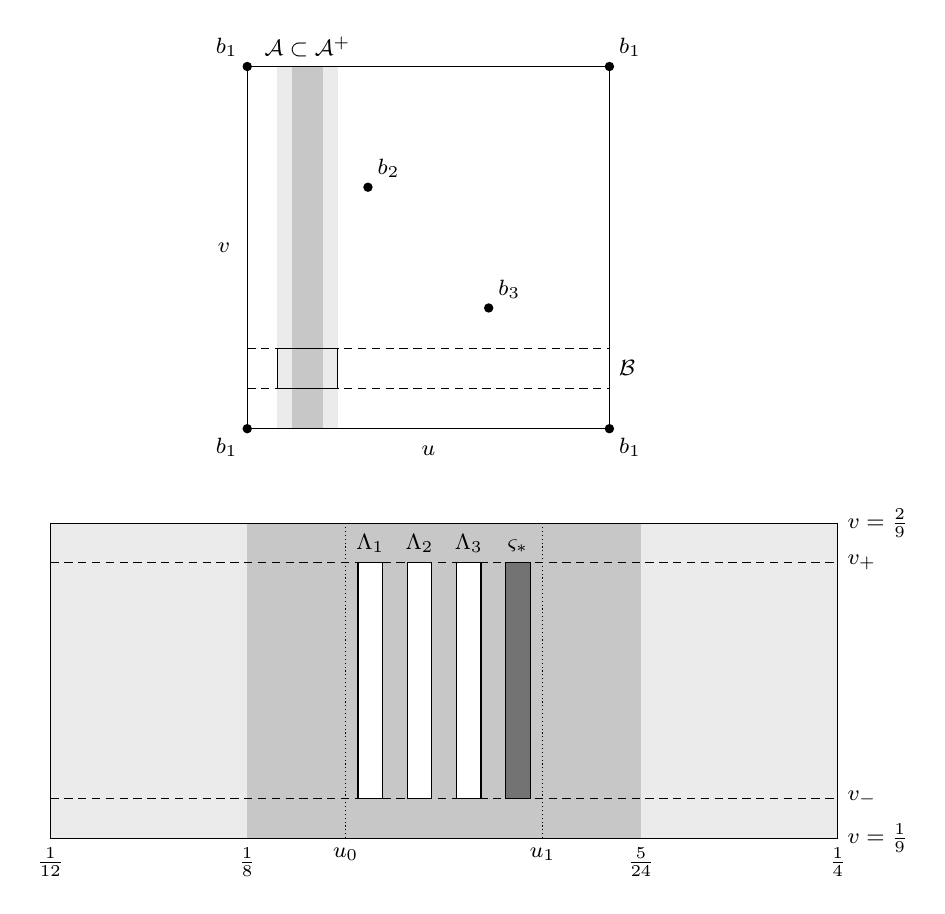
\begin{tikzpicture}[font=\footnotesize]
 \begin{scope}[scale=4.6]
  \fill[black!8] (1/12,0) rectangle (1/4,1);
  \fill[black!22] (1/8,0) rectangle (5/24,1);
  \draw[densely dashed] (0,1/9) -- (1,1/9);
  \draw[densely dashed] (0,2/9) -- (1,2/9);
  \draw (0,0) rectangle (1,1);
  \draw[thin] (1/12,1/9) rectangle (1/4,2/9);
  \foreach \p in {(0,0),(1,0),(0,1),(1,1),(1/3,2/3),(2/3,1/3)} \fill \p circle (0.013);
  \node[below left] at (0,0) {$b_1$};
  \node[below right] at (1,0) {$b_1$};
  \node[above left] at (0,1) {$b_1$};
  \node[above right] at (1,1) {$b_1$};
  \node[above right] at (1/3,2/3) {$b_2$};
  \node[above right] at (2/3,1/3) {$b_3$};
  \node[above] at (1/6,1) {$\mathcal A\subset\mathcal A^+$};
  \node[right] at (1,1/6) {$\mathcal B$};
  \node[below] at (1/2,-0.02) {$u$};
  \node[left] at (-0.02,1/2) {$v$};
 \end{scope}
 \begin{scope}[shift={(-2.5,-5.2)},x=60cm,y=36cm,shift={(-1/12,-1/9)}]
  \fill[black!8] (1/12,1/9) rectangle (1/4,2/9);
  \fill[black!22] (1/8,1/9) rectangle (5/24,2/9);
  \draw (1/12,1/9) rectangle (1/4,2/9);
  \draw[densely dashed] (1/12,1/8) -- (1/4,1/8);
  \draw[densely dashed] (1/12,5/24) -- (1/4,5/24);
  \filldraw[fill=white] (0.14844,1/8) rectangle (0.15365,5/24);
  \node[above] at (0.15104,5/24) {$\Lambda_1$};
  \filldraw[fill=white] (0.15885,1/8) rectangle (0.16406,5/24);
  \node[above] at (0.16146,5/24) {$\Lambda_2$};
  \filldraw[fill=white] (0.16927,1/8) rectangle (0.17448,5/24);
  \node[above] at (0.17188,5/24) {$\Lambda_3$};
  \filldraw[fill=black!55] (0.17969,1/8) rectangle (0.18490,5/24);
  \node[above] at (0.18229,5/24) {$\varsigma_*$};
  \draw[densely dotted] (7/48,1/9) -- (7/48,2/9);
  \draw[densely dotted] (3/16,1/9) -- (3/16,2/9);
  \node[below] at (7/48,1/9) {$u_0$};
  \node[below] at (3/16,1/9) {$u_1$};
  \node[below] at (1/8,1/9) {$\frac18$};
  \node[below] at (5/24,1/9) {$\frac5{24}$};
  \node[below] at (1/12,1/9) {$\frac1{12}$};
  \node[below] at (1/4,1/9) {$\frac14$};
  \node[right] at (1/4,1/8) {$v_-$};
  \node[right] at (1/4,5/24) {$v_+$};
  \node[right] at (1/4,1/9) {$v=\frac19$};
  \node[right] at (1/4,2/9) {$v=\frac29$};
 \end{scope}
\end{tikzpicture}
\caption{The handle data on the base torus $\Gamma=(\R/\Z)^2$ in the coordinates $(u,v)$ (Proposition~\ref{prop:cub-handle},
Definition~\ref{def:shd4-frame}). Top: the annuli $\mathcal A\subset\mathcal A^+$ (dark and light grey), the dual band
$\mathcal B$ (between $v=\frac19$ and $v=\frac29$, dashed) and the marked points $b_1,b_2,b_3$, where $Z_0=0$. Bottom: $\mathcal A^+\cap\mathcal B$
enlarged, dashed at $v=v_\pm$; the clock $f$ rises on $[u_0,u_1]$; the layers $\Lambda_i$ (white) and the
residual layer where $\varsigma_*$ rises (black) lie over $(l_j,r_j)\times(v_-,v_+)$, where $b>0$. Here $k=3$.}
\label{fig:shd4-handle}
\end{figure}

\begin{lemma}[The first path in the frame]\label{lem:shd4-frame-forms}
\lean{SymplecticPacking.Handle.Cubic.OmegaT_frameA, SymplecticPacking.Handle.Cubic.OmegaT_one_frameA,
SymplecticPacking.Handle.Cubic.Omega1Loc}
Over $\mathcal A^+$, $\chi_{\mathcal A}^*\Omega_t=\omega_V+\kappa_t+dp\wedge(a_{\mathcal A}+t\,\partial_p\alpha_1)$ with the positive forms
$\kappa_t$ of Lemma~\ref{lem:fer-positivity}. Over $\mathcal A$,
\[
 \chi_{\mathcal A}^*\Omega_1=\omega_V+e_h\nu+d\bigl(f(u)H^*(p)\beta\bigr).
\]
\end{lemma}

\begin{proof}
Lemma~\ref{lem:fer-positivity} in the frame of Lemma~\ref{lem:fer-frame}, and Lemma~\ref{lem:fer-alpha1}(ii) with $d\Gamma_{\rm sm}=e_h\nu$.
\end{proof}

\emph{The twist.} For $\lambda\in\R$ define on $\mathcal A\times\C$
\begin{equation}\label{eq:shd4-twist}
\begin{gathered}
 \mathcal D_\lambda(u,v,w_{\mathcal A})=\bigl(u,v,q_{\lambda f(u)}(w_{\mathcal A})\bigr),\qquad
 \mathcal D_\lambda^{-1}(u,v,w_{\mathcal A})=\bigl(u,v,q^{-1}_{\lambda f(u)}(w_{\mathcal A})\bigr),\\
 Q^\lambda_u=\lambda f'(u)\,Q_{\lambda f(u)},\qquad G_\lambda(u,w_{\mathcal A})=f(u)\,H^*\bigl(p(q_\lambda^{-1}w_{\mathcal A})\bigr),
\end{gathered}
\end{equation}
and $\mathcal D=\mathcal D_1$; these are smooth in $(\lambda,u,v,w_{\mathcal A})$, mutually inverse, fix base points and preserve $\mathcal A\times D(c)$ for $c>P_{\rm supp}$.
\lean{SymplecticPacking.Handle.Cubic.Dlam, SymplecticPacking.Handle.Cubic.DlamInv, SymplecticPacking.Handle.Cubic.Qs,
SymplecticPacking.Handle.Cubic.Glam}

\begin{lemma}[Suspension]\label{lem:shd4-suspension}
\lean{SymplecticPacking.Handle.Cubic.suspension}
On $\mathcal A\times\C$, $\mathcal D_\lambda^*\omega_V=\omega_V+d\bigl[(Q^\lambda_u\circ q_{\lambda f(u)})\,du\bigr]$ for every $\lambda$.
\end{lemma}

\begin{proof}
\Mref{Lemma}{lem:hdl-suspension}(i) with $m=1$ and $u$ for $s$: $D\mathcal D_\lambda$ fixes $\partial_v$, maps vertical $\xi$ to $Dq\,\xi$ and $\partial_u$ to $\partial_u+X_{Q^\lambda_u}$, and $q_{\lambda f(u)}$ is symplectic.
\end{proof}

\emph{Periodisation.} For a one-form $\alpha$ on $\widetilde N$ supported over $\{u_0\le u\le u_1\}$ put $\operatorname{per}(\alpha)=\sum_{m\in\Z}(T_u^m)^*\alpha$ (locally finite). It is $T_u$-invariant, equals $\alpha$ over $\{u_1-1<u<1+u_0\}$, vanishes near points with $u\notin[u_0,u_1]+\Z$, and for horizontal $\alpha$ its value at a point with $\lfloor u\rfloor=m$ is the covector of $\alpha$ at $T_u^{-m}$ of that point.
\lean{SymplecticPacking.Handle.Ush, SymplecticPacking.Handle.perJ}

\begin{construction}[The second-path primitive]\label{cons:shd4-eta}
\lean{SymplecticPacking.Handle.Cubic.etaLoc, SymplecticPacking.Handle.Cubic.eta, SymplecticPacking.Handle.Cubic.etaPer,
SymplecticPacking.Handle.Cubic.etaDot, SymplecticPacking.Handle.Cubic.OmS1}
On $\mathcal A\times\C$ let
\[
 \upsilon^{\mathcal A}_\lambda=\bigl(Q^\lambda_u\circ q_{\lambda f(u)}\bigr)\,du
 +f(u)\Bigl[H^*\bigl(p(q_\lambda^{-1}q_{\lambda f(u)}w_{\mathcal A})\bigr)-H^*\bigl(p(w_{\mathcal A})\bigr)\Bigr]\beta .
\]
Let $\upsilon_\lambda$ be the one-form on $\widetilde N$ equal to $(\chi_{\mathcal A}^{-1})^*\upsilon^{\mathcal A}_\lambda$ over $\mathcal A$ and to zero
elsewhere, let $\upsilon^{\rm per}_\lambda=\operatorname{per}(\upsilon_\lambda)$, and put
\[
 \Omega^{(1)}_\lambda=\Omega_1+d\upsilon^{\rm per}_\lambda,\qquad \dot\upsilon_\lambda=\partial_\lambda\upsilon^{\rm per}_\lambda .
\]
\end{construction}

\begin{lemma}[Properties of the second-path primitive]\label{lem:shd4-eta}
\lean{SymplecticPacking.Handle.Cubic.etaLoc_eq_zero_of_s, SymplecticPacking.Handle.Cubic.etaLoc_eq_zero_of_p,
SymplecticPacking.Handle.Cubic.eta_support, SymplecticPacking.Handle.Cubic.eta_smooth, SymplecticPacking.Handle.Cubic.eta_zero,
SymplecticPacking.Handle.Cubic.eta_horizontal, SymplecticPacking.Handle.Cubic.eta_TvE, SymplecticPacking.Handle.Cubic.etaDot_far,
SymplecticPacking.Handle.Cubic.firstStage_eq_pre}
\begin{enumerate}[label=(\alph*)]
\item $\upsilon^{\mathcal A}_\lambda$ vanishes for $u\le u_0$, for $u\ge u_1$, and for $p>P_{\rm supp}$; $\upsilon^{\mathcal A}_0=0$.
\item $\upsilon_\lambda$ and $\upsilon^{\rm per}_\lambda$ are horizontal one-forms on $\widetilde N$, smooth in $(\lambda,x)$; $\upsilon_\lambda$ is
$T_v$-invariant, $\upsilon^{\rm per}_\lambda$ is invariant under all deck maps, and $\upsilon^{\rm per}_0=0$. Both $\upsilon^{\rm per}_\lambda$ and $\dot\upsilon_\lambda$ vanish near every point with $p>P_{\rm supp}$ or with
$u\notin[u_0,u_1]+\Z$.
\item Over $\mathcal A$,
$\chi_{\mathcal A}^*\Omega^{(1)}_\lambda=\mathcal D_\lambda^*\bigl(\omega_V+e_h\nu+d(G_\lambda\beta)\bigr)$.
\end{enumerate}
\end{lemma}

\begin{proof}
(a) For $u\le u_0$, $f=f'=0$; for $u\ge u_1$, $f'=0$ and $q_\lambda^{-1}q_{\lambda f(u)}=\mathrm{id}$; for $p>P_{\rm supp}$, $Q_t=0$ near $w_{\mathcal A}$ and $q_t^{\pm1}$ fix it; at $\lambda=0$ both terms vanish.
(b) By (a) the extension by zero is smooth, and horizontal since $\chi_{\mathcal A}$ preserves base points. Its coefficients are $1$-periodic in $v$, so $T_v^*\upsilon_\lambda=\upsilon_\lambda$ by the $T_v$-equivariance of $\chi_{\mathcal A}$; $\operatorname{per}$ gives $T_u$-invariance, preserving $T_v$-invariance as $T_u,T_v$ commute. Supports follow from (a) and the properties of $\operatorname{per}$, also for $\partial_\lambda$.
(c) Over $\mathcal A$, $\upsilon^{\rm per}_\lambda=\upsilon_\lambda$, $\mathcal D_\lambda$ preserves $\nu,\beta$ and $G_\lambda\circ\mathcal D_\lambda=f(u)H^*(p(q_\lambda^{-1}q_{\lambda f(u)}w_{\mathcal A}))$; add Lemma~\ref{lem:shd4-suspension} to Lemma~\ref{lem:shd4-frame-forms}.
\end{proof}

\begin{proposition}[The second path]\label{prop:shd4-second}
\lean{SymplecticPacking.Handle.Cubic.OmegaPreG_split, SymplecticPacking.Handle.Cubic.firstStage_nondeg,
SymplecticPacking.Handle.Cubic.OmS1_preserves, SymplecticPacking.Handle.Cubic.twist_bound,
SymplecticPacking.Handle.Cubic.Hstar_twist_nonneg}
For valid cubic data and $\lambda\in[0,1]$, the form $\Omega^{(1)}_\lambda$ is closed, invariant under all deck maps, equal to
$\Omega_1$ for $\lambda=0$, and nondegenerate at every point of $\{p<h+2\delta_m\}$.
\end{proposition}

\begin{proof}
Closedness, invariance and $\Omega^{(1)}_0=\Omega_1$ follow from Lemma~\ref{lem:shd4-eta}(b) and Lemma~\ref{lem:fer-positivity}. By invariance we check nondegeneracy over $\{u_1-1<u<1+u_0\}$. Near $u\notin[u_0,u_1]$ the form is $\Omega_1$, symplectic on $\{p<\frac13-e_h/9\}\supset\{p<h+2\delta_m\}$ (Lemmas~\ref{lem:fer-positivity}, \ref{lem:shd4-budget}(d)). Over $\mathcal A$, Lemma~\ref{lem:shd4-eta}(c) and \Mref{Lemma}{lem:hdl-top-power}(b) ($n=2$, $\sigma_{\mathcal A}=\nu$, $e=e_h$) give $(\omega_V+e_h\nu+d(G_\lambda\beta))^2=2(e_h+b(v)\,\partial_uG_\lambda)\,\omega_V\wedge\nu$ with $\partial_uG_\lambda(u,w')=f'(u)H^*(p(q_\lambda^{-1}w'))$. If $p(w_{\mathcal A})<h+2\delta_m$, then $w'=q_{\lambda f(u)}(w_{\mathcal A})$ and $q_\lambda^{-1}w'$ lie in $D(h+2\delta_m)$, where $H^*>0$ (Lemma~\ref{lem:shd4-budget}(d)); with $f',b\ge0$, $e_h>0$ the coefficient is positive.
\end{proof}

\emph{The final coefficient.} Put
$G_{\rm f}(u,w)=J(p(w))+\sum_{i=1}^k\varsigma_i(u)\,h_i(p(w))+\varsigma_*(u)\,R^*(w)$ and $A_i=J+\sum_{j<i}h_j$.
\lean{SymplecticPacking.Handle.Cubic.Gf, SymplecticPacking.Handle.Cubic.aLayer}

\begin{lemma}[The final coefficient]\label{lem:shd4-Gf}
\lean{SymplecticPacking.Handle.Cubic.contDiff_Gf, SymplecticPacking.Handle.Cubic.Gf_mono, SymplecticPacking.Handle.Cubic.Gf_low,
SymplecticPacking.Handle.Cubic.Gf_up, SymplecticPacking.Handle.Cubic.Gf_layer}
For valid cubic data, $G_{\rm f}$ is smooth on $\R\times\C$ and
\begin{enumerate}[label=(\alph*)]
\item $\partial_uG_{\rm f}=\sum_i\varsigma_i'h_i\circ p+\varsigma_*'R^*\ge0$ at every $(u,w)$ with $R^*(w)\ge0$;
\item $G_{\rm f}=J\circ p$ for $u\le l_1$, and $G_{\rm f}=K\circ p\circ q^{-1}$ for $u\ge r_*$;
\item $G_{\rm f}(u,w)=A_i(p(w))+\varsigma_i(u)h_i(p(w))$ for $l_i<u<r_i$, $1\le i\le k$.
\end{enumerate}
\end{lemma}

\begin{proof}
(a) Differentiate; $h_i>0$ (Lemma~\ref{lem:shd4-budget}(a)), $\varsigma_j'\ge0$. (b) For $u\le l_1$ all clocks vanish; for $u\ge r_*$ all equal one and $J+\sum_ih_i+R^*=K\circ p\circ q^{-1}$. (c) On $(l_i,r_i)$, $\varsigma_j=1$ for $j<i$ and $\varsigma_j=0$ for $j>i$, including $j=*$.
\end{proof}

\begin{construction}[The third-path primitive]\label{cons:shd4-xi}
\lean{SymplecticPacking.Handle.Cubic.Gdiff, SymplecticPacking.Handle.Cubic.xiA, SymplecticPacking.Handle.Cubic.JbE,
SymplecticPacking.Handle.Cubic.xi, SymplecticPacking.Handle.Cubic.xiPer, SymplecticPacking.Handle.Cubic.OmS2,
SymplecticPacking.Handle.Cubic.OmegaFinalPer, SymplecticPacking.Handle.Cubic.Ghat}
On $\mathcal A\times\C$ let $\xi^{\mathcal A}=\bigl((G_{\rm f}-G_1)\circ\mathcal D\bigr)\beta$. Let $\xi$ be the one-form on $\widetilde N$ equal to
$J(p)\beta+(\chi_{\mathcal A}^{-1})^*\bigl(\xi^{\mathcal A}-J(p)\beta\bigr)$ over $\mathcal A$ and to $J(p)\beta$ elsewhere, and put
\[
\begin{gathered}
 \xi^{\rm per}=J(p)\beta+\operatorname{per}\bigl(\xi-J(p)\beta\bigr),\qquad
 \Omega^{(2)}_\tau=\Omega^{(1)}_1+\tau\,d\xi^{\rm per},\\
 \Omega_{\rm fin}=\Omega^{(2)}_1,\qquad \hat G_\tau=(1-\tau)G_1+\tau G_{\rm f}.
\end{gathered}
\]
\end{construction}

\begin{lemma}[Properties of the third-path primitive]\label{lem:shd4-xi}
\lean{SymplecticPacking.Handle.Cubic.xi_collar, SymplecticPacking.Handle.Cubic.xi_smooth,
SymplecticPacking.Handle.Cubic.xi_horizontal, SymplecticPacking.Handle.Cubic.xi_toric_near_boundary,
SymplecticPacking.Handle.Cubic.xi_TvE, SymplecticPacking.Handle.Cubic.xiPer_deck, SymplecticPacking.Handle.Cubic.xiPer_eq_fX,
SymplecticPacking.Handle.Cubic.fX_far, SymplecticPacking.Handle.Cubic.secondStage_eq_on_A,
SymplecticPacking.Handle.Cubic.secondStage_off}
\begin{enumerate}[label=(\alph*)]
\item $\xi^{\mathcal A}=J(p)\beta$ for $u\le u_0$ and for $u\ge u_1$.
\item $\xi^{\rm per}$ is a smooth one-form on $\widetilde N$, invariant under all deck maps, of the form $\Xi\,\beta$ with $\Xi$ smooth; on
$\{p>P_{\rm supp}\}$, $\Xi$ is a function of $(u\bmod1,p)$.
\item Over $\mathcal A$, $\chi_{\mathcal A}^*\Omega^{(2)}_\tau=\mathcal D^*\bigl(\omega_V+e_h\nu+d(\hat G_\tau\beta)\bigr)$; near points with
$u\notin[u_0,u_1]+\Z$, $\Omega^{(2)}_\tau=\Omega_1+\tau J'(p)\,b(v)\,dp\wedge dv$.
\end{enumerate}
\end{lemma}

\begin{proof}
(a) For $u\le u_0$: $\mathcal D=\mathrm{id}$, $G_1=0$, $G_{\rm f}=J\circ p$. For $u\ge u_1>r_*$: $G_1\circ\mathcal D=H^*(p)$, $G_{\rm f}\circ\mathcal D=K(p)$, with difference $J(p)$.

(b) By (a), $\xi-J(p)\beta$ is supported over $[u_0,u_1]$, so $\xi$ and $\xi^{\rm per}$ are smooth multiples of $\beta$ ($\chi_{\mathcal A}$ preserves base points). Invariance follows as in Lemma~\ref{lem:shd4-eta}(b), $J(p)\beta$ being invariant as deck maps preserve $p$ and $v\bmod1$. On $\{p>P_{\rm supp}\}$, $\mathcal D=\mathrm{id}$ and $G_1,G_{\rm f}$ depend only on $(u,p)$.

(c) Over $\mathcal A$, $\chi_{\mathcal A}^*\xi^{\rm per}=\mathcal D^*((G_{\rm f}-G_1)\beta)$; add Lemma~\ref{lem:shd4-eta}(c) at $\lambda=1$. Near $u\notin[u_0,u_1]+\Z$, $\upsilon^{\rm per}_1=0$, $\xi^{\rm per}=J(p)\beta$ and $d(J(p)\beta)=J'(p)b(v)\,dp\wedge dv$.
\end{proof}

\begin{proposition}[The third path and the final form]\label{prop:shd4-third}
\lean{SymplecticPacking.Handle.Cubic.secondStage_nondeg, SymplecticPacking.Handle.Cubic.OmS2_preserves,
SymplecticPacking.Handle.Cubic.OmegaFinalPer_eq, SymplecticPacking.Handle.Cubic.OmegaFinal_eq_pullback,
SymplecticPacking.Strip.Cubic.DinvN, SymplecticPacking.Strip.Cubic.DinvN_pullback}
For valid cubic data and $\tau\in[0,1]$, $\Omega^{(2)}_\tau$ is closed, invariant under all deck maps and nondegenerate at every
point of $\{p<h+2\delta_m\}$. Over $\mathcal A$,
\[
 \chi_{\mathcal A}^*\Omega_{\rm fin}=\mathcal D^*\Omega_{\rm pre},\qquad
 (\chi_{\mathcal A}\circ\mathcal D^{-1})^*\Omega_{\rm fin}=\Omega_{\rm pre},\qquad
 \Omega_{\rm pre}=\omega_V+e_h\nu+d(G_{\rm f}\beta),
\]
and $\chi_{\mathcal A}\circ\mathcal D^{-1}$ maps $\mathcal A\times D(h)$ diffeomorphically onto $\mathcal A\times D(h)$.
\end{proposition}

\begin{proof}
Closedness and invariance follow from Proposition~\ref{prop:shd4-second} and Lemma~\ref{lem:shd4-xi}(b), so it suffices to work over $\{u_1-1<u<1+u_0\}$.

Over $\mathcal A$, Lemma~\ref{lem:shd4-xi}(c) and \Mref{Lemma}{lem:hdl-top-power}(b) give the square at $\mathcal D(x)$ as $2(e_h+b\,\partial_u\hat G_\tau)\,\omega_V\wedge\nu$, where $\partial_u\hat G_\tau=(1-\tau)\partial_uG_1+\tau\partial_uG_{\rm f}$. If $p(x)<h+2\delta_m$, the image fibre point $w'$ has $p(w')<h+2\delta_m$, so $\partial_uG_1(u,w')\ge0$ as in Proposition~\ref{prop:shd4-second}, and $\partial_uG_{\rm f}(u,w')\ge0$ by Lemmas~\ref{lem:shd4-Gf}(a) and~\ref{lem:shd4-budget}(d).

Near $u\notin[u_0,u_1]$, Lemma~\ref{lem:shd4-xi}(c) adds $dp\wedge(\text{base one-form})$ to $\Omega_1$, which changes only the mixed part in the local form of Lemma~\ref{lem:fer-positivity}; the square remains $2\omega_V\wedge\kappa_1>0$ (Lemma~\ref{lem:pre-top-power}).

The identities are Lemma~\ref{lem:shd4-xi}(c) at $\tau=1$. The last claim holds because $\mathcal D^{\pm1}$ fix base points, $q_t^{\pm1}$ preserve $D(h)$, and $\chi_{\mathcal A}$ preserves $p$.
\end{proof}

\begin{lemma}[Vanishing on the marked fibres]\label{lem:shd4-fibres}
\lean{SymplecticPacking.Handle.fibreSetH, SymplecticPacking.Handle.Cubic.alpha1E_fibre,
SymplecticPacking.Handle.Cubic.etaDot_fibre, SymplecticPacking.Handle.Cubic.xiPer_fibre,
SymplecticPacking.Handle.Cubic.xi_zero_of_bB, SymplecticPacking.Handle.Cubic.xiPer_fibre}
Let $\widetilde{\mathcal F}$ be the union of all lifts of the fibres $N_{b_1},N_{b_2},N_{b_3}$, that is, the set of points
$(u,v,w)$ with $(u,v)\in b_j+\Z^2$ for some $j$. At every point of $\widetilde{\mathcal F}$ the covectors $\alpha_1$, $\dot\upsilon_\lambda$ $(\lambda\in\R)$ and $\xi^{\rm per}$ of
$T^*\widetilde N$ are zero.
\end{lemma}

\begin{proof}
For $\alpha_1$, lift Lemma~\ref{lem:fer-alpha1-fibres} to the cover, where $\alpha_1$ is periodic. The $u$-coordinates $0,\frac13,\frac23$ of the $b_j$ avoid $[u_0,u_1]=[\frac7{48},\frac9{48}]$ mod one, so $\dot\upsilon_\lambda$ vanishes near $\widetilde{\mathcal F}$ by Lemma~\ref{lem:shd4-eta}(b). Finally, $\xi^{\rm per}=\Xi\,b(v)\,dv$ by Lemma~\ref{lem:shd4-xi}(b). The $v$-coordinates $0,\frac23,\frac13$ lie outside $[\frac18,\frac5{24}]+\Z\supset\operatorname{supp}b$ (Proposition~\ref{prop:cub-handle}(c)), so $\beta=0$ on $\widetilde{\mathcal F}$.
\end{proof}

\begin{construction}[The handle Moser map]\label{cons:shd4-moser}
\lean{SymplecticPacking.Handle.Cubic.stage0, SymplecticPacking.Handle.Cubic.stage1, SymplecticPacking.Handle.Cubic.stage2,
SymplecticPacking.Handle.clock, SymplecticPacking.Handle.moserPathB, SymplecticPacking.Handle.moserVariationB,
SymplecticPacking.Handle.concat3B, SymplecticPacking.Handle.Cubic.handleData, SymplecticPacking.Handle.Cubic.handleParams,
SymplecticPacking.Handle.solve4, SymplecticPacking.Handle.cutoffChi, SymplecticPacking.Handle.boxFieldP,
SymplecticPacking.Handle.Cubic.handlePhi, SymplecticPacking.Handle.Cubic.handlePhiInv}
The three stages are
\[
 (\Omega^{(0)}_s,\mathfrak v^{(0)}_s)=(\Omega_s,\alpha_1),\qquad
 (\Omega^{(1)}_s,\mathfrak v^{(1)}_s)=(\Omega^{(1)}_s,\dot\upsilon_s),\qquad
 (\Omega^{(2)}_s,\mathfrak v^{(2)}_s)=(\Omega^{(2)}_s,\xi^{\rm per}),
\]
with matching endpoints $\Omega^{(0)}_1=\Omega^{(1)}_0$ and $\Omega^{(1)}_1=\Omega^{(2)}_0$. With the clocks $\sigma_i(t)=S(9t-3i-1)$,
$i=0,1,2$, which move only on $[\frac{3i+1}9,\frac{3i+2}9]$, put
\[
 \Omega^{\rm M}_t=\Omega^{(0)}_{\sigma_0(t)}+\sum_{i=1,2}\bigl(\Omega^{(i)}_{\sigma_i(t)}-\Omega^{(i)}_0\bigr),\qquad
 \mathfrak v_t=\sum_{i=0}^2\sigma_i'(t)\,\mathfrak v^{(i)}_{\sigma_i(t)} .
\]
On $U=\{p<h+2\delta_m\}$ let $Y_t$ be the field with $\iota_{Y_t}\Omega^{\rm M}_t=-\mathfrak v_t$; in the coordinates
$(\operatorname{Re}w,\operatorname{Im}w,u,v)$ it is the adjugate solution of a $4\times4$ skew system. With the moment cutoff
\[
 \mathfrak c(p)=S\Bigl(\frac{h+\frac74\delta_m-p}{\delta_m/4}\Bigr),
\]
which equals one for $p\le h+\frac32\delta_m$ and zero for $p\ge h+\frac74\delta_m$, let $\widehat Y_t=\mathfrak c(p)Y_t$, extended by zero.
The handle Moser map $\Phi$ is the time-one map of $\widehat Y$ from time $0$, and $\Phi^{-1}$ is its inverse.
\end{construction}

\begin{proposition}[The handle Moser map]\label{prop:shd4-moser}
\lean[needed]{SymplecticPacking.Handle.Cubic.handleMoser, SymplecticPacking.Handle.handle_moser_global,
SymplecticPacking.Handle.Cubic.OmegaT_toric, SymplecticPacking.Handle.Cubic.etaDot_far,
SymplecticPacking.Handle.Cubic.d1_xiPer_toric, SymplecticPacking.Handle.Cubic.handleData_pres}
For valid cubic data, $\Phi$ and $\Phi^{-1}$ are mutually inverse $C^\infty$ diffeomorphisms of $\widetilde N$, and:
\begin{enumerate}[label=(\alph*)]
\item $\Phi^*\Omega_{\rm fin}=\Omega_0$ and $(\Phi^{-1})^*\Omega_0=\Omega_{\rm fin}$ at every point of $\{p\le h+\delta_m\}$;
\item for every $c>P_{\rm supp}$, $\Phi$ and $\Phi^{-1}$ map each of $\{p\le c\}$, $\{p<c\}$, $\{p=c\}$ onto itself;
\item $\Phi$ and $\Phi^{-1}$ fix every point of $\widetilde{\mathcal F}$;
\item $\Phi$ and $\Phi^{-1}$ commute with every deck map.
\end{enumerate}
Moreover $\Phi=\Phi_2\circ\Phi_1\circ\Phi_0$, where $\Phi_i$ is the time-one map of the cut stage field $\mathfrak c(p)Y^{(i)}_s$,
$\iota_{Y^{(i)}_s}\Omega^{(i)}_s=-\mathfrak v^{(i)}_s$.
\end{proposition}

\begin{proof}
\emph{Hypotheses.} On $[\frac{3i+1}9,\frac{3i+2}9]$ only $\sigma_i$ moves, so $\Omega^{\rm M}_t=\Omega^{(i)}_{\sigma_i(t)}$ there; $\Omega^{\rm M}_t=\Omega_0$ for $t\le\frac19$ and $\Omega^{\rm M}_t=\Omega_{\rm fin}$ for $t\ge\frac89$. Hence $\Omega^{\rm M}_t$ is closed and nondegenerate on $U$, by Lemma~\ref{lem:fer-positivity}, Lemma~\ref{lem:shd4-budget}(d) and Propositions~\ref{prop:shd4-second},~\ref{prop:shd4-third}.

The pair is smooth on $\R\times\widetilde N$, with $\partial_t\Omega^{\rm M}_t=d\mathfrak v_t$ and $\mathfrak v_t=0$ for $t\notin(0,1)$. By Lemma~\ref{lem:pre-moser}(a), $Y$ is smooth on $\R\times U$, hence $\widehat Y$ is smooth on $\R\times\widetilde N$. All stage data and $\mathfrak c(p)$ are deck invariant.

\emph{Toric band.} Let $R=2\pi(-y\partial_x+x\partial_y)$ with $w=x+iy$, so that $\iota_R\Omega_0=-dp$ (Lemma~\ref{lem:fer-positivity}). On $U'=\{P_{\rm supp}<p<h+2\delta_m\}$ we have $\iota_R\Omega^{\rm M}_t=-dp$ and $\mathfrak v_t(R)=0$: $\alpha_1$ is horizontal with $\iota_Rd\alpha_1=0$, $\upsilon^{\rm per}_s$ and $\dot\upsilon_s$ vanish near $U'$ (Lemma~\ref{lem:shd4-eta}(b)), and $\xi^{\rm per}=\Xi(u\bmod1,p)\,b(v)\,dv$ on $U'$. Lemma~\ref{lem:pre-moser}(d) then gives $dp(\widehat Y_t)=0$ on $\{p>P_{\rm supp}\}$. Moreover $\widehat Y=0$ for $p\ge h+\frac74\delta_m$.

\emph{Completeness.} By Lemma~\ref{lem:pre-moser}(g), $du(\widehat Y_t)$ and $dv(\widehat Y_t)$ are deck invariant, hence $|du(\widehat Y_t)|+|dv(\widehat Y_t)|\le C_b$, the maximum over $[0,1]\times[0,1]^2\times\bar D(h+\frac74\delta_m)$; also $\widehat Y_t=0$ for $t\notin[0,1]$. By the toric band, an integral curve through $x$ stays in $\{p\le\max(p(x),h)\}$ with base displacement at most $C_b$, so the flow is global and smooth.

\emph{Conclusions.}
(b) follows from $dp(\widehat Y_t)=0$ on $\{p>P_{\rm supp}\}$.
(a) Since $P_{\rm supp}<h$, curves from $\{p\le h+\delta_m\}$ stay there, and $\{p<h+\frac32\delta_m\}$ is invariant. There $\mathfrak c=1$, so Lemma~\ref{lem:pre-moser}(b) gives $(\Phi^*\Omega^{\rm M}_1)_x=(\Omega^{\rm M}_0)_x$; the inverse identity follows as $\Phi^{-1}$ preserves $\{p\le h+\delta_m\}$.
(c) By Lemma~\ref{lem:shd4-fibres}, $\widehat Y_t=0$ on $\widetilde{\mathcal F}$; apply Lemma~\ref{lem:pre-moser}(c).
(d) is Lemma~\ref{lem:pre-moser}(g).

\emph{Decomposition.} Each stage pair is deck invariant and satisfies $\iota_R\Omega^{(i)}_s=-dp$ and $\mathfrak v^{(i)}_s(R)=0$ on $U'$, so the same argument gives a global flow $\Phi^{(i)}_s$ of $\mathfrak c(p)Y^{(i)}_s$; set $\Phi_i=\Phi^{(i)}_1$. On $[\frac{3i+1}9,\frac{3i+2}9]$ we have $\widehat Y_t=\sigma_i'(t)\mathfrak c(p)Y^{(i)}_{\sigma_i(t)}$, so $t\mapsto\Phi^{(i)}_{\sigma_i(t)}(x)$ is an integral curve of $\widehat Y$; elsewhere $\widehat Y_t=0$. Uniqueness and Lemma~\ref{lem:pre-moser}(f) give $\Phi=\Phi_2\circ\Phi_1\circ\Phi_0$.
\end{proof}

Equivalently, let $\Phi_A$ ($A\ge0$) be the time-one map of $\widehat Y$ times a product cutoff in $(u,v)$ equal to one on $\{|u|,|v|\le A+C_b+2\}$. Then $\Phi(x)=\Phi_A(x)$ for $A=|u(x)|+|v(x)|$, by the base speed bound.
\lean{SymplecticPacking.Handle.boxCut, SymplecticPacking.Handle.Cb, SymplecticPacking.Handle.boxL,
SymplecticPacking.Handle.PhiB, SymplecticPacking.Handle.PhiG, SymplecticPacking.Handle.PhiGInv,
SymplecticPacking.Handle.lfield_boxField, SymplecticPacking.Handle.LField.flowFrom_isSol, SymplecticPacking.Handle.flowFrom_box_eq}

\emph{Layer maps.} Work on the layer $\Lambda_i=\{l_i<u<r_i,\ \frac18<v<\frac5{24},\ p<h\}$ (frame coordinates). Let $T(v)=\int_{1/8}^vb$, a diffeomorphism $(\frac18,\frac5{24})\to(0,1)$ with $dT=\beta$ and inverse $v(T)$. Set $\ell(T)=e_h/b(v(T))$ and
\[
 x_i(u,T,p)=(u-l_i)\,\ell(T)+\varsigma_i(u)\,h_i(p).
\]
Since $\partial_ux_i=\ell+\varsigma_i'h_i>0$, $x_i=0$ at $u=l_i$ and $x_i>h_i(p)$ at $u=r_i$, there is a unique root $u=\sigma_i(x,T,p)\in(l_i,r_i)$ for $0<x<h_i(p)$, $0<T<1$.

For $1\le i\le k$ put $\bar\rho_i=(\rho_i+a_i)/2$, $\delta_i=a_i-\bar\rho_i$ and $\hat\rho_i=\bar\rho_i+\delta_i/4$. For $(z_{\rm b},z_{\rm f})\in\Bo(\hat\rho_i)\subset\C^2$, write $(x,T)=\Psi_{\delta_i}(z_{\rm b})$ (Proposition~\ref{prop:hdl-strip}) and $p=\pi|z_{\rm f}|^2$, and define
\[
 E_i(z_{\rm b},z_{\rm f})=\Bigl(\sigma_i(x,T,p),\ v(T),\ e^{-2\pi iTA_i'(p)}z_{\rm f}\Bigr),\qquad
 f^N_i=\Phi^{-1}\circ\chi_{\mathcal A}\circ\mathcal D^{-1}\circ E_i .
\]
\lean{SymplecticPacking.Strip.Cubic.ell, SymplecticPacking.Strip.Cubic.layerX, SymplecticPacking.Strip.Cubic.layerRoot,
SymplecticPacking.Strip.Cubic.shear, SymplecticPacking.Strip.Cubic.srcMap, SymplecticPacking.Strip.Cubic.layerMap,
SymplecticPacking.Strip.Cubic.layerMap_eq, SymplecticPacking.Strip.Cubic.fN}

\begin{proposition}[The four-dimensional embeddings into the cover]\label{prop:shd4-maps}
\lean[needed]{SymplecticPacking.Strip.Cubic.x_lt_hi, SymplecticPacking.Strip.Cubic.layer_form,
SymplecticPacking.Strip.Cubic.shear_pullback, SymplecticPacking.Strip.Cubic.layerMap_symplectic,
SymplecticPacking.Strip.Cubic.layerMap_mem_annulus, SymplecticPacking.Strip.Cubic.layerMap_injective,
SymplecticPacking.Strip.Cubic.layerMap_disjoint, SymplecticPacking.Strip.Cubic.layerMap_compact,
SymplecticPacking.Strip.Cubic.fN_mem, SymplecticPacking.Strip.Cubic.fN_smooth, SymplecticPacking.Strip.Cubic.fN_symplectic,
SymplecticPacking.Strip.Cubic.fN_eq_imp, SymplecticPacking.Strip.Cubic.fN_disjoint,
SymplecticPacking.Strip.Cubic.fN_avoid_fibres, SymplecticPacking.Strip.Cubic.fN_eq_imp,
SymplecticPacking.Embed.Cubic.fcap_eq_imp}
Let the cubic data be valid and $1\le i,j\le k$. Then $\rho_i<\bar\rho_i<\hat\rho_i<a_i$, and:
\begin{enumerate}[label=(\alph*)]
\item $f^N_i$ is defined and smooth on $\Bo(\hat\rho_i)$, with values in $\{p<h\}\setminus\widetilde{\mathcal F}$, and
$(f^N_i)^*\Omega_0=\omega_0$;
\item $f^N_i$ is injective, $f^N_i(\Bo(\hat\rho_i))\cap f^N_j(\Bo(\hat\rho_j))=\varnothing$ for $i\ne j$, and $f^N_i(B(\bar\rho_i))$ is compact;
\item if $f^N_i(X)=T\,f^N_j(X')$ for a deck map $T$, then $T=\mathrm{id}$, $i=j$ and $X=X'$.
\end{enumerate}
\end{proposition}

\begin{proof}
Let $\varpi=\pi|z_{\rm b}|^2$, so $\varpi+p<\hat\rho_i$. By Proposition~\ref{prop:hdl-strip} and Lemma~\ref{lem:shd4-budget}(a),
\[
0<x<\varpi+\tfrac{\delta_i}2<a_i-p-\tfrac{\delta_i}4<h_i(p),\qquad p<a_i<h,
\]
so $E_i$ maps $\Bo(\hat\rho_i)$ into $\Lambda_i$.

Since $\ell\,b=e_h$, $e_h\nu=\ell\,du\wedge dT$, and by Lemma~\ref{lem:shd4-Gf}(c), $d(G_{\rm f}\beta)=(\varsigma_i'h_i\,du+dA_i+\varsigma_i\,dh_i)\wedge dT$ on $\Lambda_i$; hence $\Omega_{\rm pre}=\omega_V+dx_i\wedge dT+dA_i(p)\wedge dT$ there.

Now $E_i$ is the composite of $\Psi_{\delta_i}\times\mathrm{id}$, the shear of Lemma~\ref{lem:hdl-shear} with $A=A_i$, and the inverse of $(u,v,w_{\mathcal A})\mapsto(x_i,T,w_{\mathcal A})$ (the periodic counterpart of the layer maps of~\cite{SongHD}). By Proposition~\ref{prop:hdl-strip} and Lemma~\ref{lem:hdl-shear}, $E_i$ is a diffeomorphism onto an open subset of $\Lambda_i$ with $E_i^*\Omega_{\rm pre}=\omega_0$.

(a) By Proposition~\ref{prop:shd4-third}, $\chi_{\mathcal A}\mathcal D^{-1}$ maps $\Lambda_i$ into $\mathcal A\times D(h)$ and pulls $\Omega_{\rm fin}$ back to $\Omega_{\rm pre}$; by Proposition~\ref{prop:shd4-moser}(a),(b), $\Phi^{-1}$ preserves $\{p<h\}$ and pulls $\Omega_0$ back to $\Omega_{\rm fin}$ there. Composing gives $(f^N_i)^*\Omega_0=\omega_0$. The point $\chi_{\mathcal A}\mathcal D^{-1}E_i(X)$ lies over $\mathcal A$, which misses $\widetilde{\mathcal F}$, and $\Phi^{\pm1}$ fix $\widetilde{\mathcal F}$ pointwise (Proposition~\ref{prop:shd4-moser}(c)), so $f^N_i$ misses $\widetilde{\mathcal F}$.

(b) $E_i$ is injective, and the images of different $E_i$ lie over the disjoint intervals $(l_i,r_i)$. The maps $\chi_{\mathcal A}\mathcal D^{-1}$ and $\Phi^{-1}$ are injective and common to all $i$. The closed ball is compact.

(c) By Proposition~\ref{prop:shd4-moser}(d), $y=\chi_{\mathcal A}\mathcal D^{-1}E_i(X)$ and $y'=\chi_{\mathcal A}\mathcal D^{-1}E_j(X')$ satisfy $y=Ty'$. Both lie over $(\frac18,\frac5{24})^2$, so $T=\mathrm{id}$, and (b) gives $i=j$ and $X=X'$.
\end{proof}

\begin{remark}[The four-dimensional embeddings]\label{rem:shd-four}
\lean{SymplecticPacking.Embed.Cubic.fcap, SymplecticPacking.Embed.Cubic.fcapV, SymplecticPacking.Branch2.CubicData.fcapGen,
SymplecticPacking.Handle.Cubic.handleMoser, SymplecticPacking.Strip.fN, SymplecticPacking.Embed.Cubic.fcap,
SymplecticPacking.Branch2.embeddings2, SymplecticPacking.Branch2.embeddingsEq, SymplecticPacking.Branch2.CubicData.ofParams}
By Proposition~\ref{prop:shd4-maps}(a),(c) the maps $f^N_i$ satisfy the hypotheses of Theorem~\ref{thm:cub-transfer}, and
the four-dimensional embeddings are
$f^{\rm cap}_i=b_{\rm ball}\circ\mathcal T_{\rm u}\circ\mathsf N\circ f^N_i$ on $\Bo(\hat\rho_i)$. The equal branch uses these maps for the data of
Remark~\ref{rem:rtc-equal}: $\rho_i=\rho$, $a_i=a$, $K(p)=(3\sqrt k-9)p$, and $(q_t)$ the isotopy of
Theorem~\ref{thm:pll-inner}, with the recorded capacities of Remark~\ref{rem:rtc-recorded}; the valid cubic data
of~\cite{SongHD} use the same maps. The strip constants are
the four-dimensional values of Definition~\ref{def:str-enlarged}; only the disc-to-strip map of Proposition~\ref{prop:str-strip}
is taken from \S\ref{sec:str}.
\end{remark}

\subsection{The shear and the strip map}\label{sec:shd-shear}

The layer maps of \S\ref{sec:shd-four}, and those of the higher-dimensional handle~\cite{SongHD}, use the
following two maps.

\begin{lemma}[Multi-angle shear]\label{lem:hdl-shear}
\lean{OAI.PackingSufficiencySupport.Hamiltonian.toricSuspension,
OAI.PackingSufficiencySupport.Hamiltonian.toricSuspensionInverse_smooth,
OAI.PackingSufficiencySupport.Hamiltonian.toricSuspension_pullback,
OAI.PackingSufficiencySupport.Hamiltonian.toricSuspensionInverse_left,
OAI.PackingSufficiencySupport.Hamiltonian.toricSuspensionInverse_right}
Let $A$ be a smooth function on an open set $W\subset\R^m$ and $\mathrm{Sh}_A(x,T,w)=(x,T,\mathrm{Sh}_{A,T}(w))$, where
\[
 \mathrm{Sh}_{A,T}(w)_j=\exp\big(-2\pi i\,T\,\partial_jA(p(w))\big)\,w_j\qquad(1\le j\le m),
\]
on $\{(x,T,w):p(w)\in W\}\subset\R^2\times\C^m$. Then $\mathrm{Sh}_A$ is a diffeomorphism of this set onto itself, preserves
$p$, $x$ and $T$, and
\[
 \mathrm{Sh}_A^*\big(\omega_V+dx\wedge dT+dA(p)\wedge dT\big)=\omega_V+dx\wedge dT .
\]
\end{lemma}

\begin{proof}
$\mathrm{Sh}_{A,T}$ multiplies each $w_j$ by a unimodular factor smooth in $(T,p(w))$, so it preserves $p$; the same formula with $+2\pi i$ is a smooth inverse, also on the coordinate axes. Where all $w_j\ne0$, write $w_j=\sqrt{p_j/\pi}\,e^{2\pi i\theta_j}$; then $\mathrm{Sh}_{A,T}$ is $\theta_j\mapsto\theta_j-T\partial_jA(p)$ and
\[
\mathrm{Sh}_A^*\omega_V=\omega_V-dA\wedge dT-T\sum_{j,k}\partial_{jk}A\,dp_j\wedge dp_k=\omega_V-dA\wedge dT .
\]
The Hessian term vanishes by symmetry, and $dx\wedge dT$ and $dA(p)\wedge dT$ are unchanged. The identity extends to the axes by continuity.
\end{proof}

\begin{proposition}[Disc-to-strip map]\label{prop:hdl-strip}
\lean{SymplecticPacking.Strip.psiStrip, SymplecticPacking.Strip.psiStrip_smooth,
 SymplecticPacking.Strip.psiStrip_symplectic, SymplecticPacking.Strip.psiStrip_bijOn,
 SymplecticPacking.Strip.psiStrip_x_pos, SymplecticPacking.Strip.psiStrip_x_lt}
\uses{prop:str-strip}
For every $\delta>0$ there is an explicit smooth diffeomorphism
$\Psi_\delta\colon\C\to(0,\infty)\times(0,1)$, $z\mapsto(x,T)$, with $\Psi_\delta^*(dx\wedge dT)=\omega_\C$ and
\[
 0<x<\pi|z|^2+\frac\delta2\qquad\text{for all }z\in\C .
\]
\end{proposition}

The map is $\Psi_\delta=F\circ\mathsf T^{-1}\circ\mathsf D$, with $\varepsilon=\delta/\pi$: $F(u,v)=(X(u),Y(v))$ inverts the square roots of the Morse functions $x+\varepsilon^2/(4x)-\varepsilon$ on $(0,\infty)$ and $\varepsilon\,[(2\sqrt{T(1-T)})^{-1}-1]$ on $(0,1)$, and $\mathsf T$, $\mathsf D$ are the explicit rotation and radial area normalisations of the density $X'(u)Y'(v)$. The estimate holds because the level set of energy $\mathcal E$ encloses area at least $\mathcal E-\varepsilon(\frac\pi2-1)$ and lies in $\{x<\mathcal E+\varepsilon\}$ (Proposition~\ref{prop:str-strip}). Some excess is unavoidable, since no area-preserving map takes the closed disc of area $a$ into $\{0<x<a\}\times(0,1)$; the excess $\delta/2$ serves all concentric discs at once.
